\chapter{FPGA} % Main chapter title
\label{FPGA} % For referencing the chapter elsewhere, use \ref{Chapter1} 

\section{Einleitung}
Ein FPGA (Field Programmable Gate Array) ist ein integrierter Schaltkreis, in den eine beliebige logische Schaltung programmiert werden kann. Diese Schaltungsstruktur wird mittels vorgefertiger Logikblöcke im Chip gespeichert, ohne dass die Hardware selbst verändert werden muss.

Die umgesetzte Logik der meisten FPGAs kann außerdem beliebig oft durch
das Laden einer neuen Konfigurationsdatei geändert werden. Sie sind
gegenüber fest in Hardware umgesetzten Lösungen (z. B. ASICs) damit sehr
flexibel. FPGAs eignen sich somit insbesondere für die Prototyping- und
Testphase von Hardwareprojekten.~\cite[S. 8]{SynthesisFPGA}

\section{Technik}
\paragraph{Configurable Logic Blocks.} FPGAs bestehen aus einem zweidimensionalen Array von programmierbaren Logikblöcken, den \emph{Configurable Logic Blocks} (CLB). \cite[S. 11]{Chu} Der genaue Aufbau ist dabei herstellerabhängig, sie bestehen aber mindestens aus einer Look-Up Table (LUT) und einem Flipflop. \cite[S. 8]{SynthesisFPGA}

\begin{figure} [ht]
  \centering
  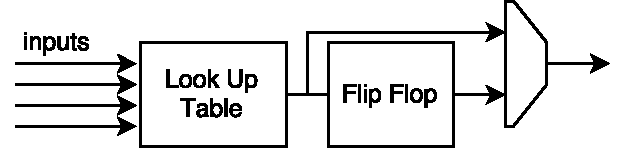
\includegraphics[width=0.5\textwidth]{Figures/clb}
  \caption{Aufbau eines simplen Configurable Logic Blocks.}
  \label{fig:clb}
\end{figure}

\paragraph{Look-Up Tables.} Look-Up Tables haben $n$ Eingänge (meistens zwischen 4 und 6) und einen Ausgang. Sie sind so konfigurierbar, dass sie eine beliebige Binärfunktion umsetzen. Zu diesem Zweck enthält jede LUT $2^n$ Speicherzellen, in denen die Werte für jede beliebige Eingangssignalkombination abgelegt werden können. Sie sind so verschaltet, dass eine bestimmte Eingangskombination zur Ausgabe des Wertes der dazugehörigen Speicherzelle führt. \cite[S. 12f.]{Chu} Durch Neubelegung dieser Speicherzellen kann die umgesetzte Logik des FPGAs beliebig verändert werden.

\paragraph{Flipflops.} Durch den fest verbauten D-Flipflop kann die Ausgabe des Logikblocks nicht nur direkt weitergegeben, sondern auch zwischengespeichert werden. Dadurch lassen sich rückgekoppelte Logiken (Schaltwerke) realisieren. \cite[S. 13]{Chu}

\paragraph{Verbindungen.} Die einzelnen CLBs sind wiederum mit
konfigurierbaren Verbindungen verdrahtet. Diese Schaltung ist durch
ein Gitter aus Leitungen realisiert, an deren Kreuzungspunkten die Signalverteilung mittels eines programmierbaren Schalters beliebig konfiguriert werden kann. \cite[S. 12]{Chu}

\section{Verwendete Hardware}
Für dieses Projekt wurde das \emph{Nexys 4}-Board mit einem Xilinx
\emph{Artix-7}-FPGA verwendet. Dieser enthält $101440$ Logic-Cells, die
in $15850$ Logic-Slices organisiert sind. Diese sind wiederum aus
jeweils vier LUTs mit sechs Inputs und acht Flipflops aufgebaut. Der
FPGA erlaubt die Implementierung von bis zu $1188$ kB Distributed RAM
(durch die Logikbausteine implementierter RAM). Außerdem steht
$4860$ Kbit Block-RAM zur Verfügung. Das Board wird mit einem internen 
100Mhz Takt versorgt. \cite{Artix}
